\documentclass[handout, aspectratio=169]{beamer}
%\documentclass[aspectratio=169]{beamer}
\usepackage[orientation=landscape,size=custom,width=16,height=9,scale=0.4,debug]{beamerposter} 

\usepackage[english]{babel}
\usepackage{metalogo}
\usepackage{listings}
% \usepackage{fontspec}
\usepackage{tikz}
\usepackage{graphicx}
\usepackage{subcaption}
%%%%%%%%%%%%%%%%%%%%%%%%%%%%%%%%%%%%%%%%%%%%%%%%%%%%%%%%%%%%%%%%%%%%%%%%%%%%%%%%%%%%%%%%
%%%%%%%%%%%%%%%%%%%%%%%%%%%%%%%%%%%%%%%%%%%%%%%%%%%%%%%%%%%%%%%%%%%%%%%%%%%%%%%%%%%%%%%%
%%%%%%%%%%%%%%%%%%%%%%%%%%%%%%%%%%%%%%%%%%%%%%%%%%%%%%%%%%%%%%%%%%%%%%%%%%%%%%%%%%%%%%%%
\usepackage{xcolor}
\definecolor{BK}{HTML}{3b3838}
\definecolor{Blue}{RGB}{88, 105, 225}
\newcommand{\BK}[1]{\color{BK} #1}
\newcommand{\URed}[1]{\color{URed} #1}
\newcommand{\white}[1]{\color{white} #1}
\newcommand{\Orange}[1]{\color{QOrange} #1}
\newcommand{\blue}[1]{\color{blue} #1}
\newcommand{\Blue}[1]{\color{Blue} #1}
\newcommand{\red}[1]{\color{red} #1}
\newcommand{\gray}[1]{\color{gray} #1}
\newcommand{\orange}[1]{\color{orange} #1}
\usepackage{accents}
\newcommand\thickbar[1]{\accentset{\rule{.4em}{.8pt}}{#1}}
\newcommand{\ubar}[1]{\underaccent{\bar}{#1}}
\newcommand{\hatbar}[1]{\bar{\hat{#1}}}
\newcommand{\hatubar}[1]{\underaccent{\bar}{\hat{#1}}}
\newcommand{\ul}[1]{\underline{#1}}
\newcommand{\ol}[1]{\overline{#1}}
%%%%%%%%%%%%%%%%%%%%%%%%%%%%%%%%%%%%%%%%%%%%%%%%%%%%%%%%%%%%%%%%%%%%%%%%%%%%%%%%%%%%%%%%
\newcommand{\bO}[1]{\bf \Orange #1}
%%%%%%%%%%%%%%%%%%%%%%%%%%%%%%%%%%%%%%%%%%%%%%%%%%%%%%%%%%%%%%%%%%%%%%%%%%%%%%%%%%%%%%%%
%%%%%%%%%%%%%%%%%%%%%%%%%%%%%%%%%%%%%%%%%%%%%%%%%%%%%%%%%%%%%%%%%%%%%%%%%%%%%%%%%%%%%%%%
\newcommand{\YBox}[3]{
\begin{center}
\begin{minipage}{#1\linewidth}
\begin{exampleblock}{#2}
    #3
\end{exampleblock}
\end{minipage}
\end{center}
}

\newcommand{\OBox}[3]{
\begin{center}
\begin{minipage}{#1\linewidth}
\begin{block}{#2}
    #3
\end{block}
\end{minipage}
\end{center}
}

\newcommand{\Columns}[4]{
\begin{columns}
\begin{column}{#1\textwidth}
#2
\end{column}
\begin{column}{#3\textwidth}  %%<--- here
#4
\end{column}
\end{columns}
}
%%%%% NEW MATH DEFINITIONS %%%%%

\usepackage{amsmath,amsfonts,bm}
\usepackage{amssymb}

%%%%%%%%%%%%%%%%%%%%%%%%%%%%%%%%%%%%%%%%%%%%%%%%%%%%%%%%%%%%%%%%%%%%%%%%%%%%%%%%
%%%%%%%%%%%%%%%%%%%%%%%%%%%%%%%%%%%%%%%%%%%%%%%%%%%%%%%%%%%%%%%%%%%%%%%%%%%%%%%%
\usepackage{natbib}
\usepackage{ulem}
% \usepackage{cite}
\usepackage{amsmath,amssymb,amsfonts}
\usepackage{algorithm,algorithmicx,algpseudocode}
\usepackage{graphicx}
% \usepackage{subcaption}
\usepackage{mwe}
\usepackage{textcomp}
\usepackage{xcolor}
\usepackage{dsfont}
\usepackage{bbm}
% Mark sections of captions for referring to divisions of figures
\newcommand{\figleft}{{\em (Left)}}
\newcommand{\figcenter}{{\em (Center)}}
\newcommand{\figright}{{\em (Right)}}
\newcommand{\figtop}{{\em (Top)}}
\newcommand{\figbottom}{{\em (Bottom)}}
\newcommand{\captiona}{{\em (a)}}
\newcommand{\captionb}{{\em (b)}}
\newcommand{\captionc}{{\em (c)}}
\newcommand{\captiond}{{\em (d)}}

% Highlight a newly defined term
\newcommand{\newterm}[1]{{\bf #1}}


% Figure reference, lower-case.
\def\figref#1{figure~\ref{#1}}
% Figure reference, capital. For start of sentence
\def\Figref#1{Figure~\ref{#1}}
\def\twofigref#1#2{figures \ref{#1} and \ref{#2}}
\def\quadfigref#1#2#3#4{figures \ref{#1}, \ref{#2}, \ref{#3} and \ref{#4}}
% Section reference, lower-case.
\def\secref#1{section~\ref{#1}}
% Section reference, capital.
\def\Secref#1{Section~\ref{#1}}
% Reference to two sections.
\def\twosecrefs#1#2{sections \ref{#1} and \ref{#2}}
% Reference to three sections.
\def\secrefs#1#2#3{sections \ref{#1}, \ref{#2} and \ref{#3}}
% Reference to an equation, lower-case.
\def\eqref#1{equation~\ref{#1}}
% Reference to an equation, upper case
\def\Eqref#1{Equation~\ref{#1}}
% A raw reference to an equation---avoid using if possible
\def\plaineqref#1{\ref{#1}}
% Reference to a chapter, lower-case.
\def\chapref#1{chapter~\ref{#1}}
% Reference to an equation, upper case.
\def\Chapref#1{Chapter~\ref{#1}}
% Reference to a range of chapters
\def\rangechapref#1#2{chapters\ref{#1}--\ref{#2}}
% Reference to an algorithm, lower-case.
\def\algref#1{algorithm~\ref{#1}}
% Reference to an algorithm, upper case.
\def\Algref#1{Algorithm~\ref{#1}}
\def\twoalgref#1#2{algorithms \ref{#1} and \ref{#2}}
\def\Twoalgref#1#2{Algorithms \ref{#1} and \ref{#2}}
% Reference to a part, lower case
\def\partref#1{part~\ref{#1}}
% Reference to a part, upper case
\def\Partref#1{Part~\ref{#1}}
\def\twopartref#1#2{parts \ref{#1} and \ref{#2}}

\def\ceil#1{\lceil #1 \rceil}
\def\floor#1{\lfloor #1 \rfloor}
\def\1{\bm{1}}
\newcommand{\train}{\mathcal{D}}
\newcommand{\valid}{\mathcal{D_{\mathrm{valid}}}}
\newcommand{\test}{\mathcal{D_{\mathrm{test}}}}

\def\eps{{\epsilon}}


% Random variables
\def\reta{{\textnormal{$\eta$}}}
\def\ra{{\textnormal{a}}}
\def\rb{{\textnormal{b}}}
\def\rc{{\textnormal{c}}}
\def\rd{{\textnormal{d}}}
\def\re{{\textnormal{e}}}
\def\rf{{\textnormal{f}}}
\def\rg{{\textnormal{g}}}
\def\rh{{\textnormal{h}}}
\def\ri{{\textnormal{i}}}
\def\rj{{\textnormal{j}}}
\def\rk{{\textnormal{k}}}
\def\rl{{\textnormal{l}}}
% rm is already a command, just don't name any random variables m
\def\rn{{\textnormal{n}}}
\def\ro{{\textnormal{o}}}
\def\rp{{\textnormal{p}}}
\def\rq{{\textnormal{q}}}
\def\rr{{\textnormal{r}}}
\def\rs{{\textnormal{s}}}
\def\rt{{\textnormal{t}}}
\def\ru{{\textnormal{u}}}
\def\rv{{\textnormal{v}}}
\def\rw{{\textnormal{w}}}
\def\rx{{\textnormal{x}}}
\def\ry{{\textnormal{y}}}
\def\rz{{\textnormal{z}}}

% Random vectors
\def\rvepsilon{{\mathbf{\epsilon}}}
\def\rvtheta{{\mathbf{\theta}}}
\def\rva{{\mathbf{a}}}
\def\rvb{{\mathbf{b}}}
\def\rvc{{\mathbf{c}}}
\def\rvd{{\mathbf{d}}}
\def\rve{{\mathbf{e}}}
\def\rvf{{\mathbf{f}}}
\def\rvg{{\mathbf{g}}}
\def\rvh{{\mathbf{h}}}
\def\rvu{{\mathbf{i}}}
\def\rvj{{\mathbf{j}}}
\def\rvk{{\mathbf{k}}}
\def\rvl{{\mathbf{l}}}
\def\rvm{{\mathbf{m}}}
\def\rvn{{\mathbf{n}}}
\def\rvo{{\mathbf{o}}}
\def\rvp{{\mathbf{p}}}
\def\rvq{{\mathbf{q}}}
\def\rvr{{\mathbf{r}}}
\def\rvs{{\mathbf{s}}}
\def\rvt{{\mathbf{t}}}
\def\rvu{{\mathbf{u}}}
\def\rvv{{\mathbf{v}}}
\def\rvw{{\mathbf{w}}}
\def\rvx{{\mathbf{x}}}
\def\rvy{{\mathbf{y}}}
\def\rvz{{\mathbf{z}}}

% Elements of random vectors
\def\erva{{\textnormal{a}}}
\def\ervb{{\textnormal{b}}}
\def\ervc{{\textnormal{c}}}
\def\ervd{{\textnormal{d}}}
\def\erve{{\textnormal{e}}}
\def\ervf{{\textnormal{f}}}
\def\ervg{{\textnormal{g}}}
\def\ervh{{\textnormal{h}}}
\def\ervi{{\textnormal{i}}}
\def\ervj{{\textnormal{j}}}
\def\ervk{{\textnormal{k}}}
\def\ervl{{\textnormal{l}}}
\def\ervm{{\textnormal{m}}}
\def\ervn{{\textnormal{n}}}
\def\ervo{{\textnormal{o}}}
\def\ervp{{\textnormal{p}}}
\def\ervq{{\textnormal{q}}}
\def\ervr{{\textnormal{r}}}
\def\ervs{{\textnormal{s}}}
\def\ervt{{\textnormal{t}}}
\def\ervu{{\textnormal{u}}}
\def\ervv{{\textnormal{v}}}
\def\ervw{{\textnormal{w}}}
\def\ervx{{\textnormal{x}}}
\def\ervy{{\textnormal{y}}}
\def\ervz{{\textnormal{z}}}

% Random matrices
\def\rmA{{\mathbf{A}}}
\def\rmB{{\mathbf{B}}}
\def\rmC{{\mathbf{C}}}
\def\rmD{{\mathbf{D}}}
\def\rmE{{\mathbf{E}}}
\def\rmF{{\mathbf{F}}}
\def\rmG{{\mathbf{G}}}
\def\rmH{{\mathbf{H}}}
\def\rmI{{\mathbf{I}}}
\def\rmJ{{\mathbf{J}}}
\def\rmK{{\mathbf{K}}}
\def\rmL{{\mathbf{L}}}
\def\rmM{{\mathbf{M}}}
\def\rmN{{\mathbf{N}}}
\def\rmO{{\mathbf{O}}}
\def\rmP{{\mathbf{P}}}
\def\rmQ{{\mathbf{Q}}}
\def\rmR{{\mathbf{R}}}
\def\rmS{{\mathbf{S}}}
\def\rmT{{\mathbf{T}}}
\def\rmU{{\mathbf{U}}}
\def\rmV{{\mathbf{V}}}
\def\rmW{{\mathbf{W}}}
\def\rmX{{\mathbf{X}}}
\def\rmY{{\mathbf{Y}}}
\def\rmZ{{\mathbf{Z}}}

% Elements of random matrices
\def\ermA{{\textnormal{A}}}
\def\ermB{{\textnormal{B}}}
\def\ermC{{\textnormal{C}}}
\def\ermD{{\textnormal{D}}}
\def\ermE{{\textnormal{E}}}
\def\ermF{{\textnormal{F}}}
\def\ermG{{\textnormal{G}}}
\def\ermH{{\textnormal{H}}}
\def\ermI{{\textnormal{I}}}
\def\ermJ{{\textnormal{J}}}
\def\ermK{{\textnormal{K}}}
\def\ermL{{\textnormal{L}}}
\def\ermM{{\textnormal{M}}}
\def\ermN{{\textnormal{N}}}
\def\ermO{{\textnormal{O}}}
\def\ermP{{\textnormal{P}}}
\def\ermQ{{\textnormal{Q}}}
\def\ermR{{\textnormal{R}}}
\def\ermS{{\textnormal{S}}}
\def\ermT{{\textnormal{T}}}
\def\ermU{{\textnormal{U}}}
\def\ermV{{\textnormal{V}}}
\def\ermW{{\textnormal{W}}}
\def\ermX{{\textnormal{X}}}
\def\ermY{{\textnormal{Y}}}
\def\ermZ{{\textnormal{Z}}}

% Vectors
\def\vxi{{\bm{\xi}}}

\def\vzero{{\bm{0}}}
\def\vone{{\bm{1}}}
\def\vmu{{\bm{\mu}}}
\def\vtheta{{\bm{\theta}}}
\def\va{{\bm{a}}}
\def\vb{{\bm{b}}}
\def\vc{{\bm{c}}}
\def\vd{{\bm{d}}}
\def\ve{{\bm{e}}}
\def\vf{{\bm{f}}}
\def\vg{{\bm{g}}}
\def\vh{{\bm{h}}}
\def\vi{{\bm{i}}}
\def\vj{{\bm{j}}}
\def\vk{{\bm{k}}}
\def\vl{{\bm{l}}}
\def\vm{{\bm{m}}}
\def\vn{{\bm{n}}}
\def\vo{{\bm{o}}}
\def\vp{{\bm{p}}}
\def\vq{{\bm{q}}}
\def\vr{{\bm{r}}}
\def\vs{{\bm{s}}}
\def\vt{{\bm{t}}}
\def\vu{{\bm{u}}}
\def\vv{{\bm{v}}}
\def\vw{{\bm{w}}}
\def\vx{{\bm{x}}}
\def\vy{{\bm{y}}}
\def\vz{{\bm{z}}}

% Elements of vectors
\def\evalpha{{\alpha}}
\def\evbeta{{\beta}}
\def\evepsilon{{\epsilon}}
\def\evlambda{{\lambda}}
\def\evomega{{\omega}}
\def\evmu{{\mu}}
\def\evpsi{{\psi}}
\def\evsigma{{\sigma}}
\def\evtheta{{\theta}}
\def\eva{{a}}
\def\evb{{b}}
\def\evc{{c}}
\def\evd{{d}}
\def\eve{{e}}
\def\evf{{f}}
\def\evg{{g}}
\def\evh{{h}}
\def\evi{{i}}
\def\evj{{j}}
\def\evk{{k}}
\def\evl{{l}}
\def\evm{{m}}
\def\evn{{n}}
\def\evo{{o}}
\def\evp{{p}}
\def\evq{{q}}
\def\evr{{r}}
\def\evs{{s}}
\def\evt{{t}}
\def\evu{{u}}
\def\evv{{v}}
\def\evw{{w}}
\def\evx{{x}}
\def\evy{{y}}
\def\evz{{z}}

% Matrix
\def\mA{{\bm{A}}}
\def\mB{{\bm{B}}}
\def\mC{{\bm{C}}}
\def\mD{{\bm{D}}}
\def\mE{{\bm{E}}}
\def\mF{{\bm{F}}}
\def\mG{{\bm{G}}}
\def\mH{{\bm{H}}}
\def\mI{{\bm{I}}}
\def\mJ{{\bm{J}}}
\def\mK{{\bm{K}}}
\def\mL{{\bm{L}}}
\def\mM{{\bm{M}}}
\def\mN{{\bm{N}}}
\def\mO{{\bm{O}}}
\def\mP{{\bm{P}}}
\def\mQ{{\bm{Q}}}
\def\mR{{\bm{R}}}
\def\mS{{\bm{S}}}
\def\mT{{\bm{T}}}
\def\mU{{\bm{U}}}
\def\mV{{\bm{V}}}
\def\mW{{\bm{W}}}
\def\mX{{\bm{X}}}
\def\mY{{\bm{Y}}}
\def\mZ{{\bm{Z}}}
\def\mBeta{{\bm{\beta}}}
\def\mPhi{{\bm{\Phi}}}
\def\mLambda{{\bm{\Lambda}}}
\def\mSigma{{\bm{\Sigma}}}

% Tensor
\DeclareMathAlphabet{\mathsfit}{\encodingdefault}{\sfdefault}{m}{sl}
\SetMathAlphabet{\mathsfit}{bold}{\encodingdefault}{\sfdefault}{bx}{n}
\newcommand{\tens}[1]{\bm{\mathsfit{#1}}}
\def\tA{{\tens{A}}}
\def\tB{{\tens{B}}}
\def\tC{{\tens{C}}}
\def\tD{{\tens{D}}}
\def\tE{{\tens{E}}}
\def\tF{{\tens{F}}}
\def\tG{{\tens{G}}}
\def\tH{{\tens{H}}}
\def\tI{{\tens{I}}}
\def\tJ{{\tens{J}}}
\def\tK{{\tens{K}}}
\def\tL{{\tens{L}}}
\def\tM{{\tens{M}}}
\def\tN{{\tens{N}}}
\def\tO{{\tens{O}}}
\def\tP{{\tens{P}}}
\def\tQ{{\tens{Q}}}
\def\tR{{\tens{R}}}
\def\tS{{\tens{S}}}
\def\tT{{\tens{T}}}
\def\tU{{\tens{U}}}
\def\tV{{\tens{V}}}
\def\tW{{\tens{W}}}
\def\tX{{\tens{X}}}
\def\tY{{\tens{Y}}}
\def\tZ{{\tens{Z}}}


% Graph
\def\gA{{\mathcal{A}}}
\def\gB{{\mathcal{B}}}
\def\gC{{\mathcal{C}}}
\def\gD{{\mathcal{D}}}
\def\gE{{\mathcal{E}}}
\def\gF{{\mathcal{F}}}
\def\gG{{\mathcal{G}}}
\def\gH{{\mathcal{H}}}
\def\gI{{\mathcal{I}}}
\def\gJ{{\mathcal{J}}}
\def\gK{{\mathcal{K}}}
\def\gL{{\mathcal{L}}}
\def\gM{{\mathcal{M}}}
\def\gN{{\mathcal{N}}}
\def\gO{{\mathcal{O}}}
\def\gP{{\mathcal{P}}}
\def\gQ{{\mathcal{Q}}}
\def\gR{{\mathcal{R}}}
\def\gS{{\mathcal{S}}}
\def\gT{{\mathcal{T}}}
\def\gU{{\mathcal{U}}}
\def\gV{{\mathcal{V}}}
\def\gW{{\mathcal{W}}}
\def\gX{{\mathcal{X}}}
\def\gY{{\mathcal{Y}}}
\def\gZ{{\mathcal{Z}}}

% Sets
\def\sA{{\mathbb{A}}}
\def\sB{{\mathbb{B}}}
\def\sC{{\mathbb{C}}}
\def\sD{{\mathbb{D}}}
% Don't use a set called E, because this would be the same as our symbol
% for expectation.
\def\sF{{\mathbb{F}}}
\def\sG{{\mathbb{G}}}
\def\sH{{\mathbb{H}}}
\def\sI{{\mathbb{I}}}
\def\sJ{{\mathbb{J}}}
\def\sK{{\mathbb{K}}}
\def\sL{{\mathbb{L}}}
\def\sM{{\mathbb{M}}}
\def\sN{{\mathbb{N}}}
\def\sO{{\mathbb{O}}}
\def\sP{{\mathbb{P}}}
\def\sQ{{\mathbb{Q}}}
\def\sR{{\mathbb{R}}}
\def\sS{{\mathbb{S}}}
\def\sT{{\mathbb{T}}}
\def\sU{{\mathbb{U}}}
\def\sV{{\mathbb{V}}}
\def\sW{{\mathbb{W}}}
\def\sX{{\mathbb{X}}}
\def\sY{{\mathbb{Y}}}
\def\sZ{{\mathbb{Z}}}

% Entries of a matrix
\def\emLambda{{\Lambda}}
\def\emA{{A}}
\def\emB{{B}}
\def\emC{{C}}
\def\emD{{D}}
\def\emE{{E}}
\def\emF{{F}}
\def\emG{{G}}
\def\emH{{H}}
\def\emI{{I}}
\def\emJ{{J}}
\def\emK{{K}}
\def\emL{{L}}
\def\emM{{M}}
\def\emN{{N}}
\def\emO{{O}}
\def\emP{{P}}
\def\emQ{{Q}}
\def\emR{{R}}
\def\emS{{S}}
\def\emT{{T}}
\def\emU{{U}}
\def\emV{{V}}
\def\emW{{W}}
\def\emX{{X}}
\def\emY{{Y}}
\def\emZ{{Z}}
\def\emSigma{{\Sigma}}

% entries of a tensor
% Same font as tensor, without \bm wrapper
\newcommand{\etens}[1]{\mathsfit{#1}}
\def\etLambda{{\etens{\Lambda}}}
\def\etA{{\etens{A}}}
\def\etB{{\etens{B}}}
\def\etC{{\etens{C}}}
\def\etD{{\etens{D}}}
\def\etE{{\etens{E}}}
\def\etF{{\etens{F}}}
\def\etG{{\etens{G}}}
\def\etH{{\etens{H}}}
\def\etI{{\etens{I}}}
\def\etJ{{\etens{J}}}
\def\etK{{\etens{K}}}
\def\etL{{\etens{L}}}
\def\etM{{\etens{M}}}
\def\etN{{\etens{N}}}
\def\etO{{\etens{O}}}
\def\etP{{\etens{P}}}
\def\etQ{{\etens{Q}}}
\def\etR{{\etens{R}}}
\def\etS{{\etens{S}}}
\def\etT{{\etens{T}}}
\def\etU{{\etens{U}}}
\def\etV{{\etens{V}}}
\def\etW{{\etens{W}}}
\def\etX{{\etens{X}}}
\def\etY{{\etens{Y}}}
\def\etZ{{\etens{Z}}}

% The true underlying data generating distribution
\newcommand{\pdata}{p_{\rm{data}}}
% The empirical distribution defined by the training set
\newcommand{\ptrain}{\hat{p}_{\rm{data}}}
\newcommand{\Ptrain}{\hat{P}_{\rm{data}}}
% The model distribution
\newcommand{\pmodel}{p_{\rm{model}}}
\newcommand{\Pmodel}{P_{\rm{model}}}
\newcommand{\ptildemodel}{\tilde{p}_{\rm{model}}}
% Stochastic autoencoder distributions
\newcommand{\pencode}{p_{\rm{encoder}}}
\newcommand{\pdecode}{p_{\rm{decoder}}}
\newcommand{\precons}{p_{\rm{reconstruct}}}

\newcommand{\laplace}{\mathrm{Laplace}} % Laplace distribution

\newcommand{\E}{\mathbb{E}}
\newcommand{\Ls}{\mathcal{L}}
\newcommand{\R}{\mathbb{R}}
\newcommand{\emp}{\tilde{p}}
\newcommand{\lr}{\alpha}
\newcommand{\reg}{\lambda}
\newcommand{\rect}{\mathrm{rectifier}}
\newcommand{\softmax}{\mathrm{softmax}}
\newcommand{\sigmoid}{\sigma}
\newcommand{\softplus}{\zeta}
\newcommand{\KL}{D_{\mathrm{KL}}}
\newcommand{\Var}{\mathrm{Var}}
\newcommand{\standarderror}{\mathrm{SE}}
\newcommand{\Cov}{\mathrm{Cov}}
% Wolfram Mathworld says $L^2$ is for function spaces and $\ell^2$ is for vectors
% But then they seem to use $L^2$ for vectors throughout the site, and so does
% wikipedia.
\newcommand{\normlzero}{L^0}
\newcommand{\normlone}{L^1}
\newcommand{\normltwo}{L^2}
\newcommand{\normlp}{L^p}
\newcommand{\normmax}{L^\infty}

\newcommand{\parents}{Pa} % See usage in notation.tex. Chosen to match Daphne's book.

% \DeclareMathOperator*{\argmax}{arg\,max}
% \DeclareMathOperator*{\argmin}{arg\,min}
\DeclareMathOperator{\arginf}{arg\,inf}
\DeclareMathOperator{\argmin}{arg\,min}
\DeclareMathOperator{\argmax}{arg\,max}
\DeclareMathOperator{\argsup}{arg\,sup}
\DeclareMathOperator*{\diag}{\textit{diag}}
\DeclareMathOperator*{\trace}{\textit{tr}}
\DeclareMathOperator*{\rank}{\textit{rk}}

\DeclareMathOperator{\sign}{sign}
\DeclareMathOperator{\Tr}{Tr}
\let\ab\allowbreak

\usetheme{Nord}
%%%%% \setmainfont{}
% \setmainfont{Montserrat}
% \setsansfont{Andika New Basic}
% \setmonofont{DejaVu Sans Mono}

%%%%%%%%%%%%%%%%%%%%%%%%%%%%%%%%%%%%%%%%%%%%%%%%%%%%%%%%%%%%%%%%%%%%%%%%%%%%%%%%%%%%%%%%
%%%%%%%%%%%%%%%%%%%%%%%%%%%%%%%%%%%%%%%%%%%%%%%%%%%%%%%%%%%%%%%%%%%%%%%%%%%%%%%%%%%%%%%%
\newcommand{\bs}{

\bigskip

}
\newcommand{\ms}{

\medskip

}
%%%%%%%%%%%%%%%%%%%%%%%%%%%%%
\usepackage{tcolorbox}
\newtcolorbox{mybox}{width=9cm, left=0mm,right = 0mm,top=1mm,bottom=1mm,boxsep=0mm}
\newtcolorbox{myboxL}{width=15cm, left=0mm,right = 0mm,top=1mm,bottom=1mm,boxsep=0mm}
\newtcolorbox{mybox1}{width=5.5cm, left=0mm,right = 0mm,top=1mm,bottom=1mm,boxsep=0mm,colback=BK, coltext=QOrange}

\newtcolorbox{mybox2}{width=12cm, left=0mm,right = 0mm,top=1mm,bottom=1mm,boxsep=0mm,colback=BK, coltext=QOrange}

\newtcolorbox{mybox3}{width=3cm, left=0mm,right = 0mm,top=1mm,bottom=1mm,boxsep=0mm,colback=BK, coltext=QOrange}

\newtcolorbox{mybox4}{width=11cm, left=1mm,right = 1mm,top=1mm,bottom=1mm,boxsep=0mm,colback=BK, coltext=QOrange}
%%%%%%%%%%%%%%%%%%%%%%%%%%%%%%%%%%%%%%%%%%%%%%%%%%%%%%%%%%%%%%%%%%%%%%%%%%%%%%%%%%%%%%%%
%%%%%%%%%%%%%%%%%%%%%%%%%%%%%%%%%%%%%%%%%%%%%%%%%%%%%%%%%%%%%%%%%%%%%%%%%%%%%%%%%%%%%%%%


\graphicspath{{materials/figs}}
\usepackage{relsize}
\usepackage{inputenc}
\usepackage{graphicx}
\usepackage{amsmath,amssymb}
\usepackage{booktabs}
\usepackage{tcolorbox}
\usepackage[dvipsnames]{xcolor}

\mode<presentation>
{
   \usetheme{Berlin}
    \usecolortheme{seahorse}
    \setbeamertemplate{itemize item}    
    {\color{darkgray}$\blacktriangleright$}
    \setbeamertemplate{itemize subitem}{\color{lightgray}$\blacksquare$}
}

\newcommand{\redIMP}[1]{\color{NordOrange} #1}
\newcommand{\blueIMP}[1]{\color{NordMagenta} #1}

\definecolor{greentitle}{RGB}{126,169,105}
\definecolor{redtitle}{RGB}{26,69,15}
\definecolor{bluetitle}{RGB}{30,30,100}
\definecolor{title1}{RGB}{50,50,50}


% \setbeamercolor{block title}{bg=bluetitle,fg=white}


%-----------------
%   TITLE PAGE
%-----------------
\title{Towards Resilient Tracking in Autonomous Vehicles}
\subtitle{A Distributionally Robust Input \& State Estimation Approach}
\author{Kasra Azizi, {\blue{\textbf{Kumar Anurag}}}, Wenbin Wan}
\date{Intelligent Autonomous Vehicles, May 2025}

\addtobeamertemplate{block begin}{%
  \setlength{\textwidth}{1.2\textwidth}%
}{}

\addtobeamertemplate{block alerted begin}{%
  \setlength{\textwidth}{1.2\textwidth}%
}{}

\addtobeamertemplate{block example begin}{%
  \setlength{\textwidth}{1.2\textwidth}%
}{}

\begin{document}

% --- Title Page ---
% { \usebackgroundtemplate{
\includegraphics[width=\paperwidth]{figs/titlepic.png}} % Ensure path is correct
{\usebackgroundtemplate{
\includegraphics[width=\paperwidth]{figs/titlepic.png}}
\begin{frame}[plain,noframenumbering]
  \maketitle
\end{frame}}


\section{Introduction}
\begin{frame}
    \frametitle{\smaller{Introduction: Problem \& Solution}}
    \begin{columns}[T]

        \begin{column}{0.5\textwidth}            
            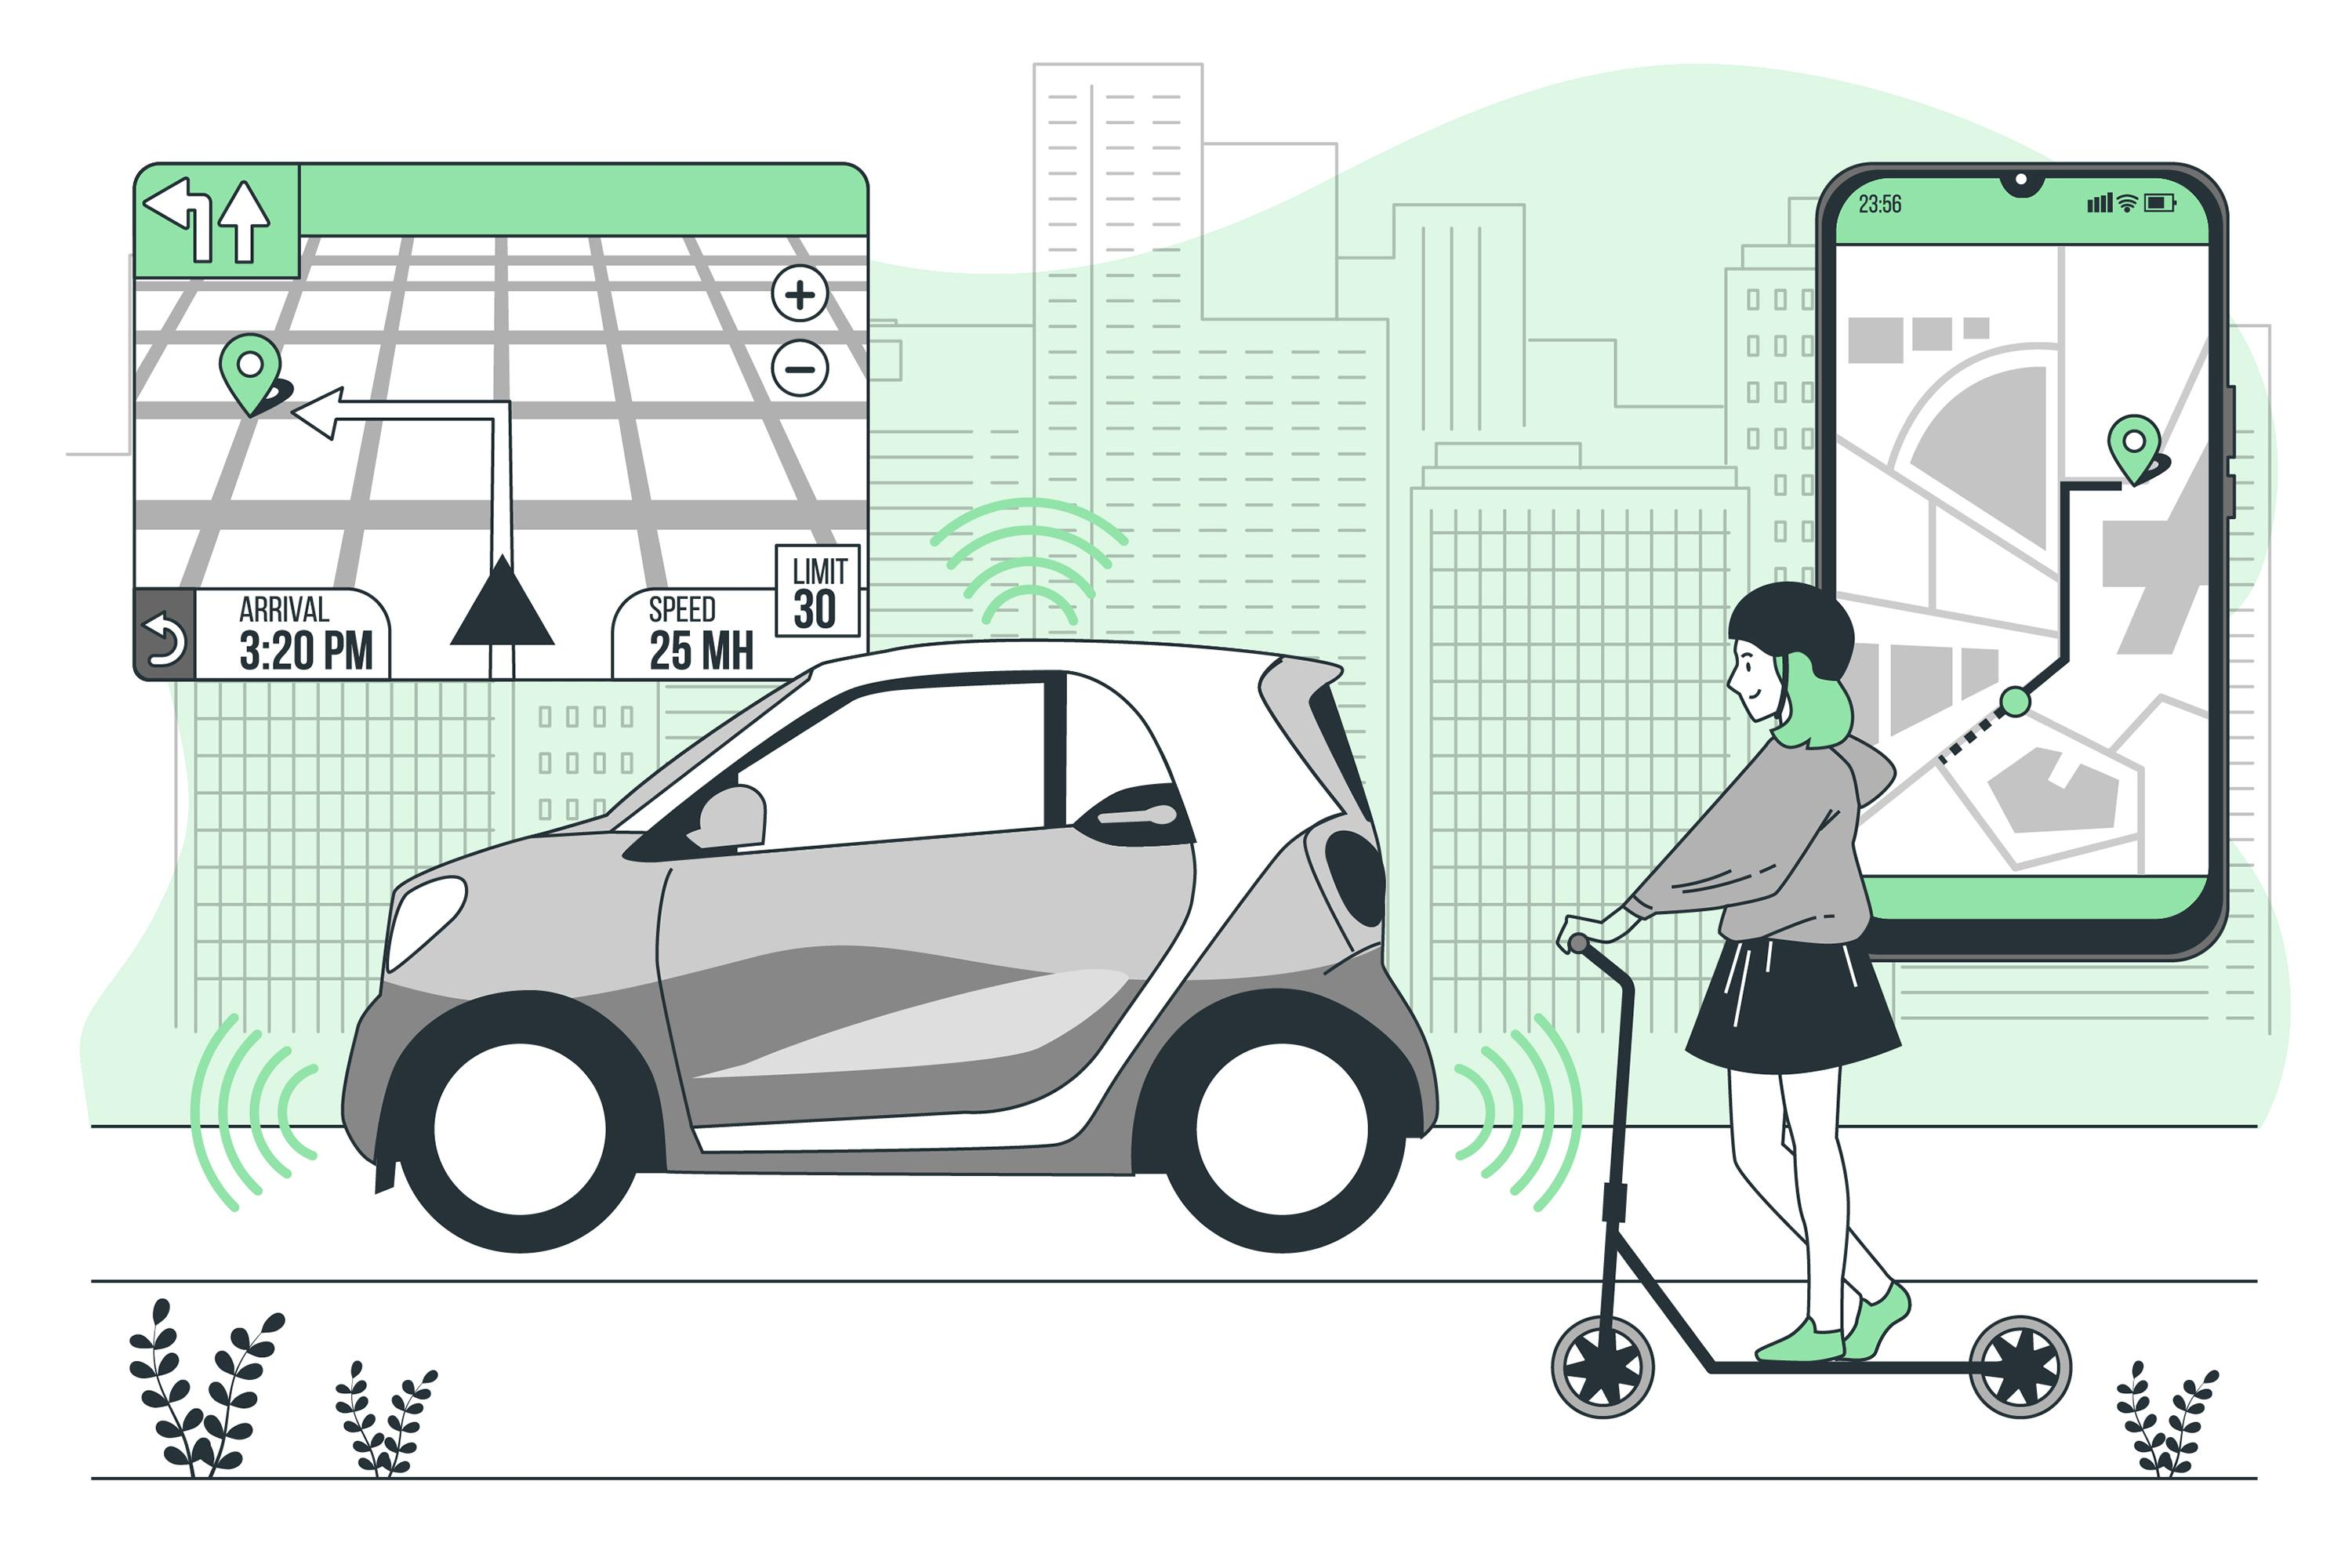
\includegraphics[width=\textwidth]{figs/car environment}   
        \end{column}

        \begin{column}{0.5\textwidth}

        \begin{tcolorbox}[colbacktitle=title1, title=\textbf{The Problem: AV Safety Imperative}]
                \begin{itemize}
                    \item<1-> \textbf{Safety} \pause
                    \item<2-> \textbf{State Data} \pause
                    \item<3-> \textbf{Noisy Measurements}
                \end{itemize}
            \end{tcolorbox}
            
            \begin{tcolorbox}[colbacktitle=title1, title=\textbf{The Solution: State Estimation}]
                \begin{itemize}
                    \item<4-> \textbf{Fuse Data} \pause
                    \item<5-> \textbf{Estimate State Using Model} \pause
                    \item<6-> \textbf{Ensure Reliability}
                \end{itemize}
            \end{tcolorbox}
        \end{column}

    \end{columns}
\end{frame}

% --- Baseline Estimators (Version 2) ---
\section{Baseline Estimators}
% --- Slide for ISE ---
\begin{frame}
  \frametitle{\smaller{Baseline: Input \& State Estimation (ISE)}}
  \begin{columns}[T]
    \begin{column}{0.65\textwidth}
        \begin{tcolorbox}[colbacktitle=greentitle, title=\textbf{Core Idea}]
            \begin{itemize}
                \item<1-> \textbf{Joint Estimation} \pause
                \item<2-> \textbf{State \& Unknown Input} \pause
                \item<3-> \textbf{Enhance Prediction} \pause
                \item<4-> \textbf{Improve Accuracy w/ Unmodeled Dynamics}
            \end{itemize}
        \end{tcolorbox}
    \end{column}
    \begin{column}{0.35\textwidth}
        \begin{tcolorbox}[colbacktitle=redtitle, title=\textbf{Key Limitation}]
             \textbf{Sensitive To:}
                \begin{itemize}
                    \item<5-> \textbf{Non-Linearity} \pause
                    \item<6-> \textbf{Non-Gaussian Noise} \pause
                    \item<7-> \textbf{Outliers}
                \end{itemize}
        \end{tcolorbox}
     \end{column}
 \end{columns}
\end{frame}

% --- Slide for DRE ---
\begin{frame}
  \frametitle{\smaller{Baseline: Distributionally Robust Estimation (DRE)}}
   \begin{columns}[T]
    \begin{column}{0.6\textwidth}
     \begin{tcolorbox}[colbacktitle=greentitle, title=\textbf{Core Idea}]
        \begin{itemize}
            \item<1-> \textbf{Robustness} \pause
            \item<2-> \textbf{Deviating Noise Distributions} \pause
            \item<3-> \textbf{Ambiguity Sets} \pause
            \item<4-> \textbf{Worst-Case Optimization}
        \end{itemize}
    \end{tcolorbox}
         \end{column}
     \begin{column}{0.4\textwidth}
    \begin{tcolorbox}[colbacktitle=redtitle,title=\textbf{Key Limitation}]
        \begin{itemize}
             \item<5-> \textbf{Sensitive to Outliers} \pause
            \item<6-> \textbf{Ignores Unknown Inputs}
        \end{itemize}
    \end{tcolorbox}
     \end{column}
 \end{columns}
\end{frame}


\section{DRISE}
% --- Problem Formulation ---
\begin{frame}[fragile] % Fragile for math
    \frametitle{\smaller{Problem Formulation}}
    \begin{columns}[T]
\begin{column}{0.6\textwidth}
    \begin{tcolorbox}[colbacktitle=title1, title=\textbf{Linear Time-Varying System with Uncertainties}]
        \textbf{System Model:}
        {\smaller
        \begin{align*}
        \vx_{k+1} &= \mA_k\vx_k + \mB_k\vu_k + \mG_k{\redIMP\vd_k} + {\redIMP\vw_k} \pause \\
        \vy_k &= \mC_k\vx_k + {\redIMP \vv_k} \pause
        \end{align*}        }
    \end{tcolorbox}
\end{column}
    \begin{column}{0.4\textwidth}
         \begin{tcolorbox}[colbacktitle=title1, title=\textbf{Key Terms:}]        
            \begin{itemize}        
                \item $\vd_k$:  Unknown Input \pause
                \item $\vw_k$:Uncertain Distribution \pause        
                \item $\vv_k$: Uncertain Distribution \pause
                 \item $\vy_k$: Outliers
            \end{itemize}
        \end{tcolorbox}
    \end{column}
\end{columns}     
\end{frame}


% ---  Building Block 1 ---
\begin{frame}[fragile]
  \frametitle{\smaller{Building Block 1: Unknown Input Estimation}}
    \begin{tcolorbox}[colbacktitle=title1, title=\textbf{Handling $\vd_k$}]
        \begin{itemize}
            \item<1-> \textbf{Problem:} Unmodeled Forces $\vd_k$. \pause
            \item<2-> \textbf{Mechanism:} Input Estimation Step in Algorithm. \pause
        \end{itemize}
        \only<4->{ % Reveal math after points
            \textbf{Key Formula:}
             {\smaller \[ \hat{\vd}_{k-1} = \mM_k(\vy_k - \mC_k\hat{\vx}_k^{-}) \] } }
    \end{tcolorbox}
    \pause
  \begin{tcolorbox}[colbacktitle=redtitle, title=\textbf{Addresses:}]
  Errors from unmodeled dynamics ($\vd_k$).
   \end{tcolorbox}
\end{frame}

% ---  Building Block 2 (DRE) ---
\begin{frame}[fragile]
  \frametitle{\smaller{Building Block 2: Distributionally Robust Estimation}}
    \begin{tcolorbox}[colbacktitle=title1, title=\textbf{Handling Noise Uncertainty ($\vw_k, \vv_k$)}]
        \begin{itemize}
            \item<1-> \textbf{Problem:} Noise Distributions Deviate. \pause
            \item<2-> \textbf{Mechanism:} Worst-Case Optimization over  Ambiguity Sets($\mathcal{F}$). \pause
        \end{itemize}
        \only<4->{ % Reveal math after points
            \textbf{Conceptual Objective:}
             {\smaller \[ \min_{\text{estimator}} \max_{P \in \mathcal{F}} E_P[\text{Error Norm}] \] }              
        }
    \end{tcolorbox}
    \begin{tcolorbox}[colbacktitle=redtitle, title=\textbf{Addresses:}]
        Performance loss from inexact noise models.
     \end{tcolorbox}
\end{frame}


% ---Building Block 3 (Robust Statistics) ---
\begin{frame}[fragile]
   \frametitle{\smaller{Building Block 3: Robust Update}}
     \begin{tcolorbox}[colbacktitle=title1, title=\textbf{Handling Measurement Outliers}]
        \begin{itemize}
            \item<1-> \textbf{Problem:} Large Measurement Outliers. \pause          
            \item<2-> \textbf{Mechanism:} Limit The Influence Function $\psi(\cdot)$. \pause
        \end{itemize}
        \only<4->{ % Reveal math after points
            \textbf{Huber influence $\psi(\cdot)$ Formula:}
            {\smaller \[ \psi(\mu) = \begin{cases} -K, & \mu \le -K \\ \mu, & |\mu| < K \\ K, & \mu \ge K \end{cases} \] } }
    \end{tcolorbox}
    \begin{tcolorbox}[colbacktitle=redtitle, title=\textbf{Addresses:}] Corruption of estimates by outliers.
    \end{tcolorbox}
 \end{frame}

% --- Slide 7: Block Diagram ---
\begin{frame}
    \frametitle{\smaller{DRISE Framework Block Diagram}}
    \begin{center}
        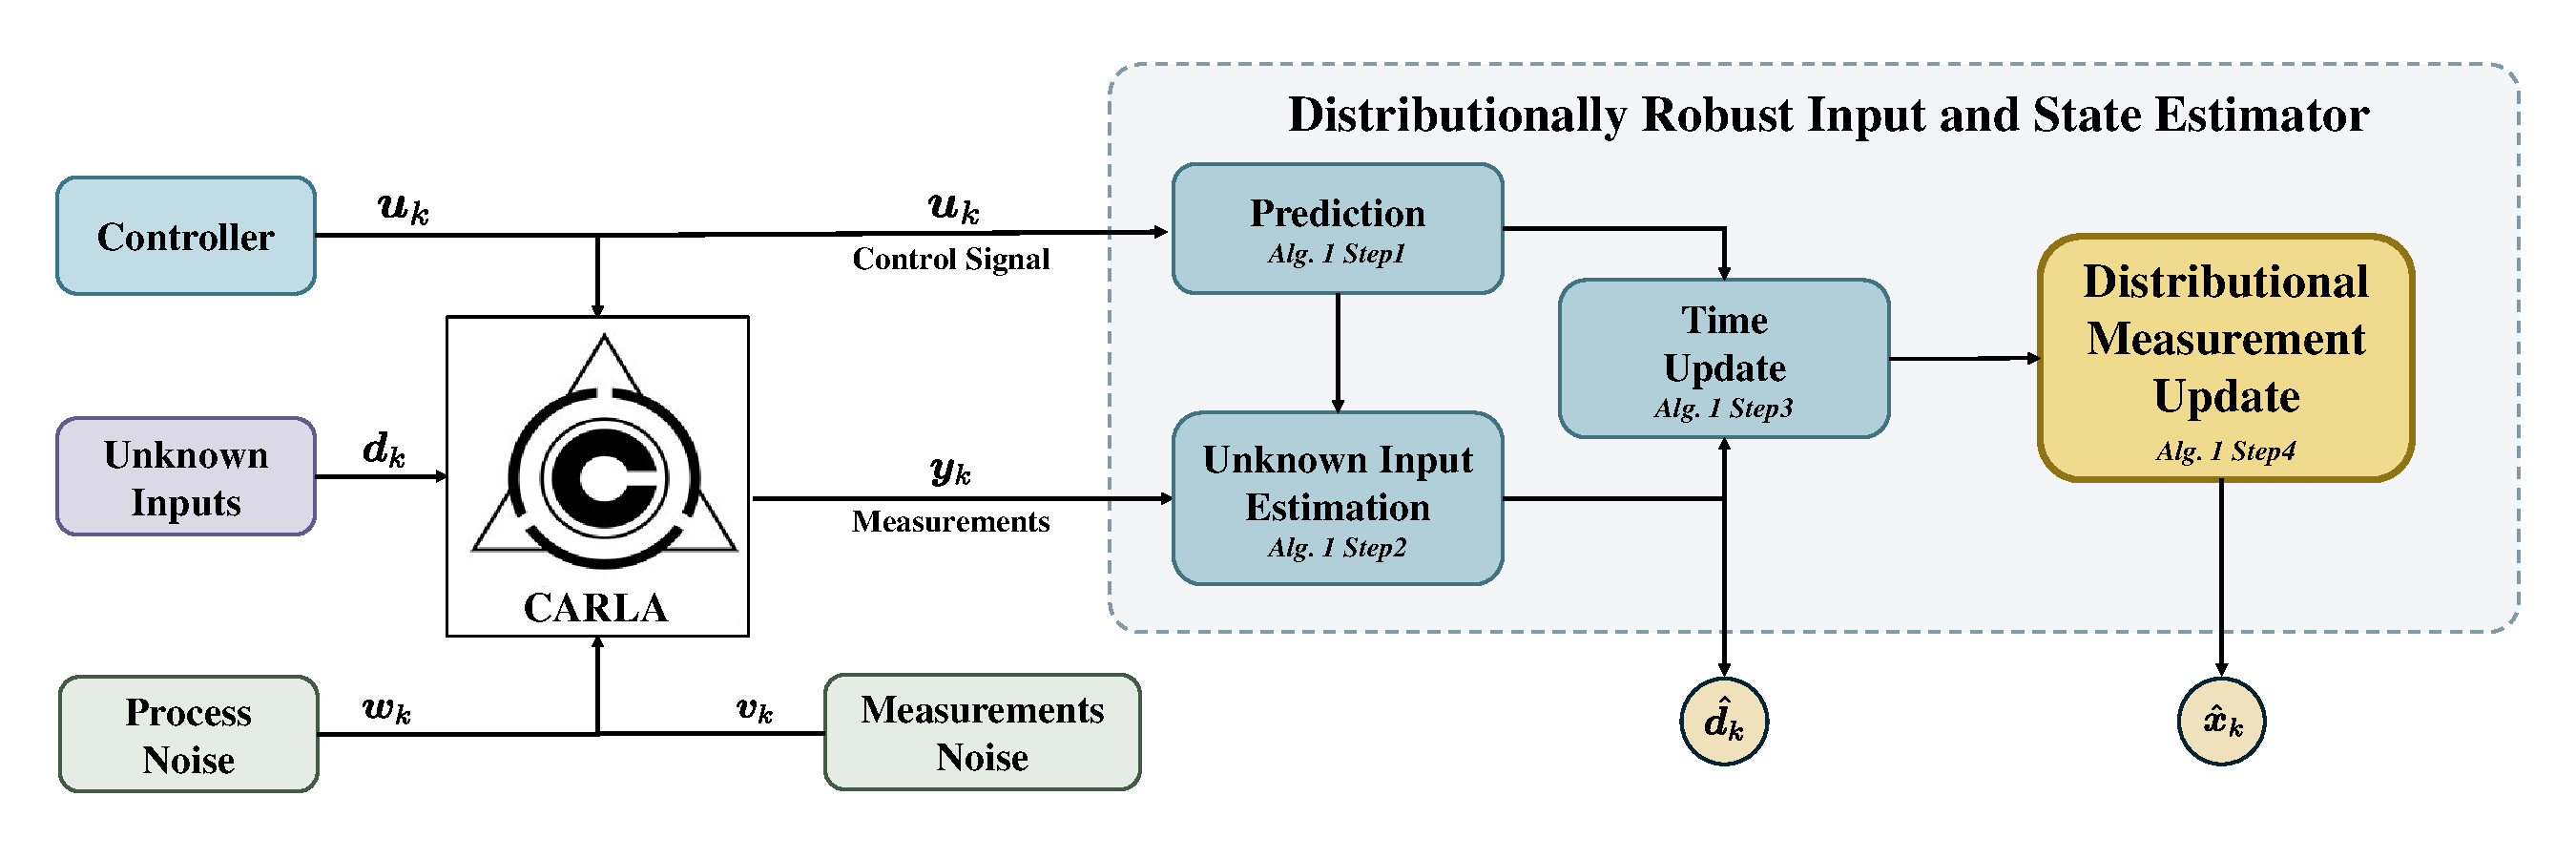
\includegraphics[width=\textwidth]{figs/BlockDiagram.pdf} % Ensure this image exists
    \end{center}
\end{frame}


% --- DRISE Algorithm Cycle Slide ---
\begin{frame}[fragile] % fragile needed for math environments
    \frametitle{\smaller{The DRISE Algorithm Cycle}} % Keep the title concise
    \begin{columns}[T]
        \begin{column}{0.55\textwidth}
            \begin{tcolorbox}[colbacktitle=title1, title=\textbf{Key Steps}]
                \begin{enumerate}
                    \item \textbf{Prediction} \vspace{0.75mm} \\ % Condensed text
                    $ \qquad \qquad \hat{\vx}_k^{-} = \mA_{k-1}\hat{\vx}_{k-1} + \mB_{k-1}\vu_{k-1} $ \pause
                    \vspace{1mm} % Add space between steps for clarity with pauses

                    \item \textbf{Input Estimation} \vspace{0.75mm} \\ % Condensed text
                    $\qquad \qquad \hat{\vd}_{k-1} = \mM_k(\vy_k - \mC_k\hat{\vx}_k^{-})$ \pause
                     \vspace{1mm}

                    \item \textbf{Time Update} \vspace{0.75mm} \\ % Condensed text
                    $ \qquad \qquad \hat{\vx}_k = \hat{\vx}_k^{-} + \mG_{k-1}\hat{\vd}_{k-1}$ \pause % State estimate after time update
                     \vspace{1mm}

                    \item \textbf{Robust Measurement Update} \vspace{0.75mm} \\ % Condensed text
                    $\qquad \qquad \hat{\vx}_k \leftarrow \hat{\vx}_k + \mL_k \psi_k(\mS_k^{-1/2}\vs_k)$ \pause
                \end{enumerate}
            \end{tcolorbox}
        \end{column}

        \begin{column}{0.45\textwidth}
            \begin{tcolorbox}[colbacktitle=title1, title=\textbf{Notation}]
                \begin{itemize}
                    \item $\mM_k$: Input est. gain. \pause
                    \item $\mL_k$: Robust gain involving ambiguity sets. \pause
                    \item $\psi_k(\cdot)$: Influence function. \pause
                    \item $\vs_k=\vy_k-\mC_k\hat{\vx}_k$: Innovation. \pause
                    \item $\mS_k$: Robust innovation covariance.%
                \end{itemize}
            \end{tcolorbox}
        \end{column}
    \end{columns}
\end{frame}


% --- Combined Simulation Setup  ---
\section{Simulation} % Ensure this section exists or adjust as needed
\begin{frame}[fragile] % fragile needed for math and possibly itemize
    \frametitle{\smaller{Simulation Setup}} % Concise title
    \begin{columns}[T] % Use T alignment

       \begin{column}{0.6\textwidth} % Adjust width for the figure
            \begin{center}
                 % Ensure this image exists and path is correct
                 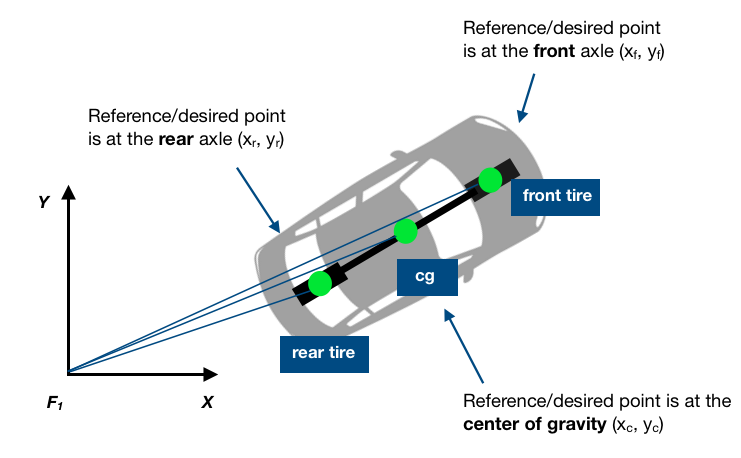
\includegraphics[width=\textwidth]{figs/kinematics.png}                 
            \end{center}
       \end{column}

        \begin{column}{0.45\textwidth} % Adjust width for the text box
            \begin{tcolorbox}[colbacktitle=title1, title=\textbf{Simulation Settings}]
                \begin{itemize}
                    \item<2-> \textbf{Model:} Kinematic Bicycle (LTV) \pause
                    \item<3-> \textbf{States $\vx_k$:} Pos, Yaw, Vels \pause
                    \item<4-> \textbf{Input $\vu_k$:} Steering, Accel \pause
                    \item<5-> \textbf{Unknown Input ($\vd_k$):} Time-Varying Signal \pause
                    \item<6-> \textbf{Noise:} Proc ($\mQ_k$), Meas ($\mR_k$)   \pause
                    \item<7-> \textbf{Outliers/Deviations:} Included in Tests \pause
                    \item<8->  \textbf{Comparison:} KF, ISE, DRE \pause
                \end{itemize}
            \end{tcolorbox}
       \end{column}
    \end{columns}
\end{frame}

%% --- Simulation ---
\begin{frame}
 \frametitle{\smaller{Simulation Environment: CARLA}}    
\begin{columns}[T]    
    \begin{column}{0.45\textwidth}
        
\includegraphics[width=\textwidth]{figs/carla.jpg}
    \end{column}
  
    \begin{column}{0.55\textwidth}
        \begin{tcolorbox}[colbacktitle=title1, title=\textbf{Testing in CARLA Simulator}]
          \begin{itemize}
            \item <1-> Open-source, high-fidelity simulator for AV research.
            \item <2-> Provides realistic urban environments, sensors, and physics.
            \item <3-> Challenging testbed for evaluating estimator performance under uncertainty.
        \end{itemize}
    \end{tcolorbox}
    \end{column}

    \end{columns}      
   \end{frame}


% --- Results Slide 1: State Estimation Error ---
\section{Results}
\begin{frame}
    \frametitle{\smaller{Results: State Estimation Error}}
    \begin{columns}[T]
        \begin{column}{0.5\textwidth} % Adjust width for figure
            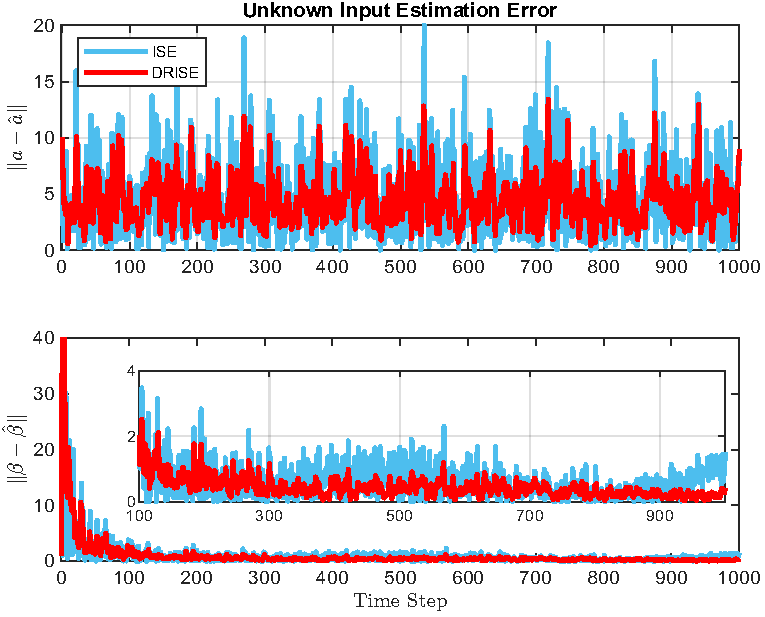
\includegraphics[width=\textwidth]{figs/AttackEstimationError.pdf} % Figure 2 (Error over time)
             \captionof{figure}{\smaller{State Estimation Error Norm}} % Add caption
        \end{column}
        \begin{column}{0.5\textwidth} % Adjust width for analysis
            \begin{tcolorbox}[colbacktitle=title1, title=\textbf{Analysis}]
                \begin{itemize}
                 \item<1-> \textbf{DRISE:} Lowest Error \pause
                    \item<2-> \textbf{KF:} Highest Error/Divergence \pause
                    \item<3-> \textbf{ISE/DRE:} Moderate Error \pause 
                \end{itemize}
            \end{tcolorbox}
        \end{column}
    \end{columns}
\end{frame}

% --- Results Slide 2: Unknown Input Error ---
\begin{frame}
    \frametitle{\smaller{Results: Unknown Input Error}}
     \begin{columns}[T]
        \begin{column}{0.5\textwidth} % Adjust width for figure
             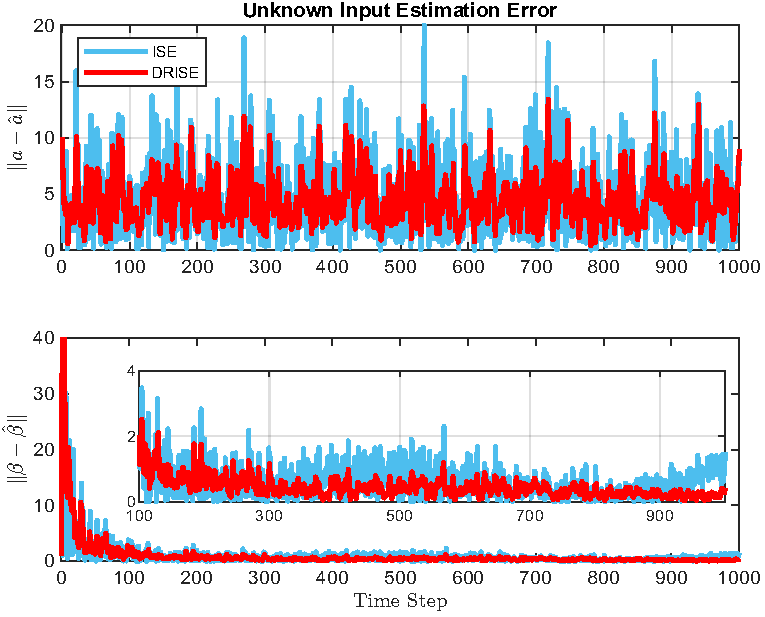
\includegraphics[width=\textwidth]{figs/AttackEstimationError.pdf} % Figure 4 (Input Error over time)
              \captionof{figure}{\smaller{Unknown Input Estimation Error}}
        \end{column}
        \begin{column}{0.5\textwidth} % Adjust width for analysis
            \begin{tcolorbox}[colbacktitle=title1, title=\textbf{Analysis}]
                \begin{itemize}
                   \item<1-> \textbf{DRISE:} Lower Error \pause
                    \item<2-> \textbf{ISE:} Higher Error \pause
                    \item<3-> \textbf{Benefit:} Robustness Aids Input Est.
                \end{itemize}
            \end{tcolorbox}
        \end{column}
    \end{columns}
\end{frame}

% --- Results Slide 3: Trajectory Tracking ---
\begin{frame}
    \frametitle{\smaller{Results: Trajectory Tracking}}
     \begin{columns}[T] % Use columns to place analysis next to figure
        \begin{column}{0.5\textwidth} % Adjust width for figure
            \centering % Center the image in its column
             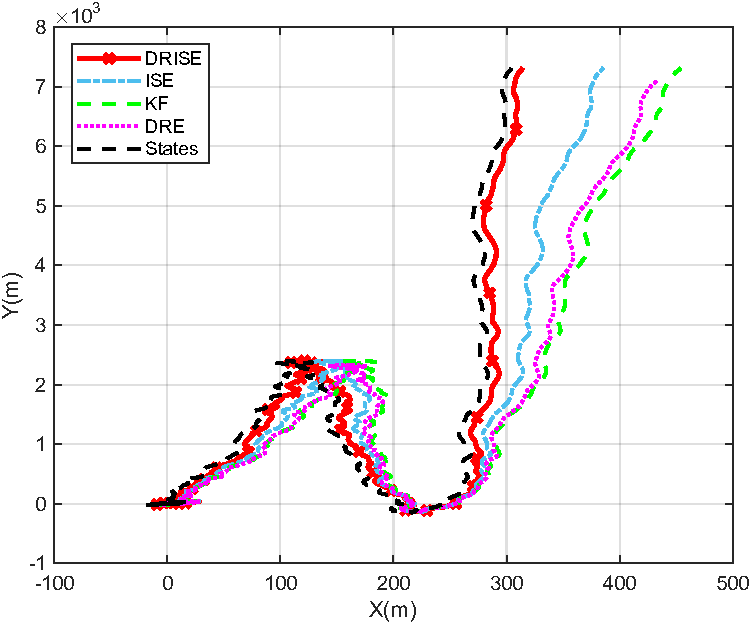
\includegraphics[width=\textwidth]{figs/Reference_Trajectory_Tracking.pdf} % Figure 3 (Trajectory)
             \captionof{figure}{\smaller{2D Trajectory Tracking}}
        \end{column}
        \begin{column}{0.5\textwidth} % Adjust width for analysis
            \begin{tcolorbox}[colbacktitle=title1, title=\textbf{Analysis}]
                \begin{itemize}
                    \item<1-> \textbf{DRISE:} Best Tracking \pause
                    \item<2-> \textbf{Others:} Show Drift \pause
                    \item<3-> \textbf{Link:} Accurate Est. $\rightarrow$ Better Tracking
                \end{itemize}
            \end{tcolorbox}
        \end{column}
    \end{columns}
\end{frame}

% --- Results Slide 4: Overall Comparison ---
\begin{frame}
    \frametitle{\smaller{Results: Overall Comparison}} % Keeping title from draft
    \begin{tcolorbox}[colbacktitle=title1, title=\textbf{DRISE Performance}] % Changed title slightly for clarity
        \begin{itemize}
            \item<1-> \textbf{Superior Accuracy}: Lowest State/Input Errors (RMSE) \pause
            \item<2-> \textbf{Robustness Confirmed}: Best performance under combined noise/outlier/input challenges \pause
            \item<3-> \textbf{Practical Benefit}: Enables Most Accurate Trajectory Tracking
        \end{itemize}
    \end{tcolorbox}
    \pause % Pause before benchmark limitations
    \begin{tcolorbox}[colbacktitle=redtitle, title=\textbf{Benchmark Limits}]
        \begin{itemize} % Using itemize instead of enumerate for consistency
            \item<5-> \textbf{KF:} Sensitive to ALL challenges \pause % Overlay number adjusted
            \item<6-> \textbf{ISE:} Sensitive to Noise/Outliers \pause
            \item<7-> \textbf{DRE:} Sensitive to Unknown Inputs/Outliers
        \end{itemize}
    \end{tcolorbox}
\end{frame}



% --- Future Work Slide  ---
\begin{frame}
\frametitle{\smaller{Future Work}} % Keep the title
    \begin{columns}[T] % Use columns for layout
        \begin{column}{0.55\textwidth} % Adjust width for left column
            \begin{tcolorbox}[colbacktitle=title1, title=\textbf{Open Questions}] % Title for the left column block
                \begin{itemize}
                    \item<1-> \textbf{Parameter Tuning:} How to optimally set $\theta$'s/K in practice? \pause % Concise open question 1
                    \item<2-> \textbf{Non-Linearity:} Extension to highly non-linear systems? \pause % Concise open question 2
                    \item<3-> \textbf{Computation:} Real-time performance on embedded hardware? % Concise open question 3
                \end{itemize}
            \end{tcolorbox}
        \end{column}

        \begin{column}{0.45\textwidth} % Adjust width for right column (more space for directions)
            \begin{tcolorbox}[colbacktitle=title1, title=\textbf{Potential Directions}] % Existing title for the right column block
                \begin{itemize} % Existing condensed items
                    \item<4-> \textbf{Explore Ambiguity Sets} \pause % Items appear after left column
                    \item<5-> \textbf{Non-Linear Systems} \pause
                    \item<6-> \textbf{Adaptive Parameter Tuning} \pause
                    \item<7-> \textbf{Other Robotics Apps}
                \end{itemize}
            \end{tcolorbox}
            \end{column}       
    \end{columns}
\end{frame}


\usebackgroundtemplate{
\includegraphics[width=\paperwidth]{figs/titlepic.png}}
\begin{frame}[plain]  
   \frametitle{\smaller{Thank You}}
    \begin{center}
        \Huge \textbf{Questions?}
    \end{center}
\end{frame}


\end{document}
 